% !TEX options=--shell-escape
\pdfobjcompresslevel=0
\documentclass[slidetop,11pt]{beamer}
\usepackage[utf8]{inputenc}
\usepackage{dsfont}
\usepackage{multirow}
\usepackage{array}
\usepackage{xcolor}
\usepackage{algorithmic}
\usepackage[plain]{algorithm}
\usepackage{ulem}
\usepackage{mathabx}
\usepackage{graphicx}
% declare the path(s) where your graphic files are
\graphicspath{{img/}}
\DeclareGraphicsExtensions{.pdf,.jpeg,.png,.eps}
\usepackage{subfig}
\usepackage{soul} % strikethrough
\usepackage{minted}


\usetheme{progressbar}
\setbeamertemplate{footline}[frame number]
\setbeamercovered{transparent}
\useinnertheme{default}

\newcommand{\mv}{{\rm  MV}}

\DeclareMathOperator*{\argmin}{\arg\!\min}
\DeclareMathOperator*{\sgn}{\text{sgn}}

\newtheorem{prop}{Property}
\newtheorem{thm}{Theorem}
\newtheorem{rem}{Remark}

\newenvironment{changemargin}[2]{%
  \begin{list}{}{% 
    \setlength{\topsep}{0pt}% 
    \setlength{\leftmargin}{#1}% 
    \setlength{\rightmargin}{#2}% 
    \setlength{\listparindent}{\parindent}% 
    \setlength{\itemindent}{\parindent}% 
    \setlength{\parsep}{\parskip}% 
  }% 
  \item[]}{\end{list}}

\makeatletter
\newcommand{\vast}{\bBigg@{3}}
\makeatother
	
\definecolor{dgreen}{rgb}{0.,0.6,0.}
\definecolor{azure}{rgb}{0.,0.5,1.}
\definecolor{bluegray}{rgb}{0.4,0.6,0.8}
\definecolor{bleu}{rgb}{0.19,0.55,0.91}

\newcommand{\semitransp}[2][30]{\color{fg!#1}#2}


\title{{\large Anomaly detection in scikit-learn} \\ {\normalfont \small{Ongoing work and future developments}}}
\author{Albert Thomas}
\institute{T\'el\'ecom ParisTech - Huawei Technologies}
\date{}


\begin{document}

\captionsetup[subfigure]{labelformat=empty}

\begin{frame}

\includegraphics[width=2.3cm]{img/scikit-learn-logo-notext.png}
% \hspace{6.7cm}
% \includegraphics[width=1cm]{img/logo_telecom.jpg}
\titlepage

\end{frame}


\begin{frame}
\frametitle{Anomaly detection}

\begin{itemize}
\item \textbf{Imbalanced classification}: anomalies and normal data available, usually highly imbalanced data set

\item \textbf{Novely detection}: normal data available, fit on normal data, then predict on unlabelled data

\item \textbf{Outlier detection}: unlabelled data only, fit \textbf{and} predict on unlabelled data. Anomalies are rare events, located in the low density regions.
\end{itemize}

\begin{center}
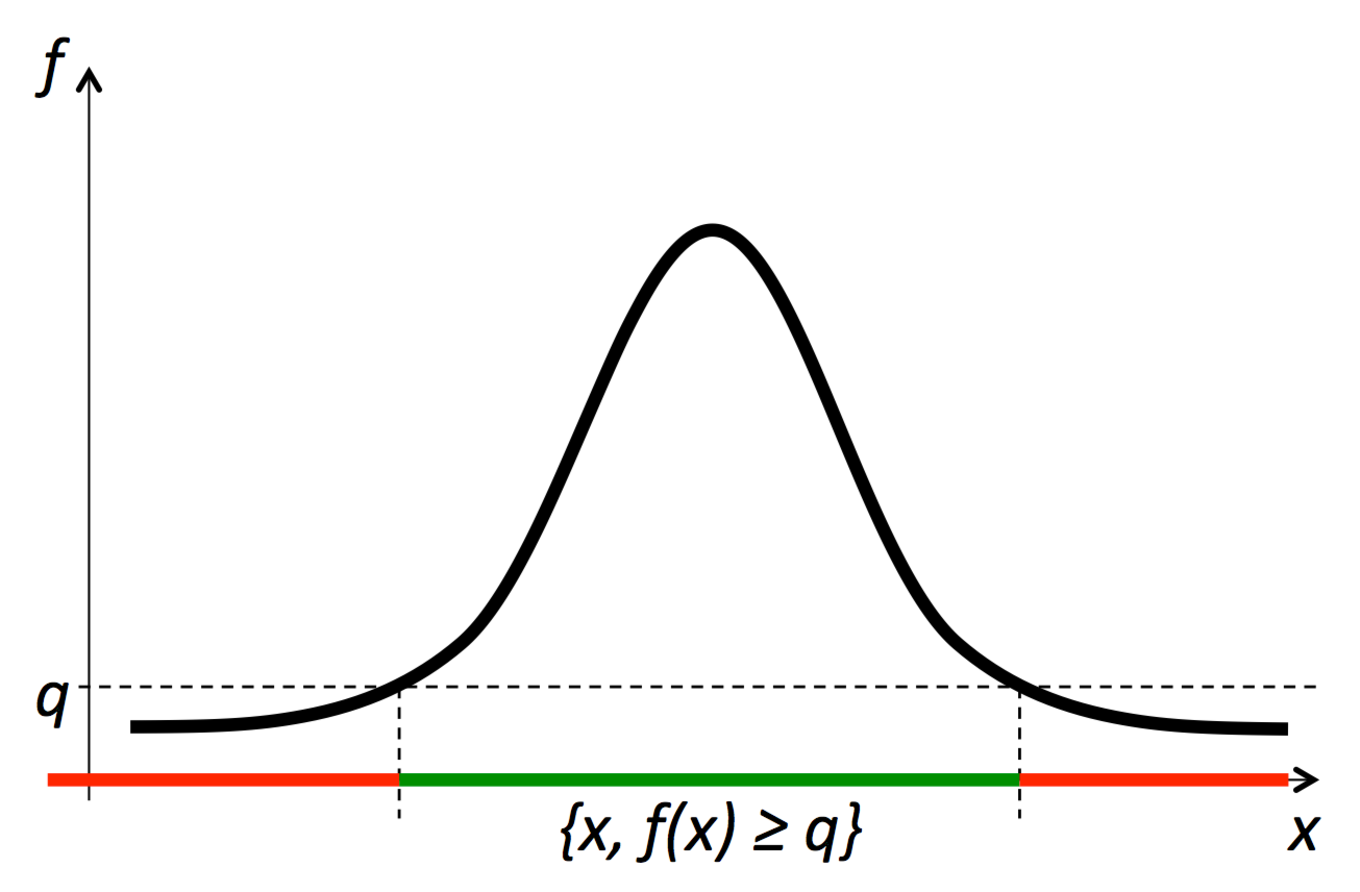
\includegraphics[width=5cm]{dls3.pdf}
\end{center}

\begin{center}
Find the \textbf{high density regions}
\end{center}

\end{frame}



\begin{frame}
\frametitle{Outlier and novelty detection algorithms}

Common approach

\vspace{0.5cm}

\begin{enumerate}
\item[1.] Learn a scoring function $s$ such that
\begin{center}
the smaller $s(x)$ the more abnormal is $x$
\end{center}

\vspace{0.5cm}

\item[2.] Threshold $s$ at an offset $q$ such that outlier/novelties are such that
\begin{equation*}
\{x, s(x) < q \}
\end{equation*}
$q$ usually depends on a \mintinline{python}{contamination} parameter
\end{enumerate}

\end{frame}


\begin{frame}\frametitle{Algorithms}
    
\begin{center}
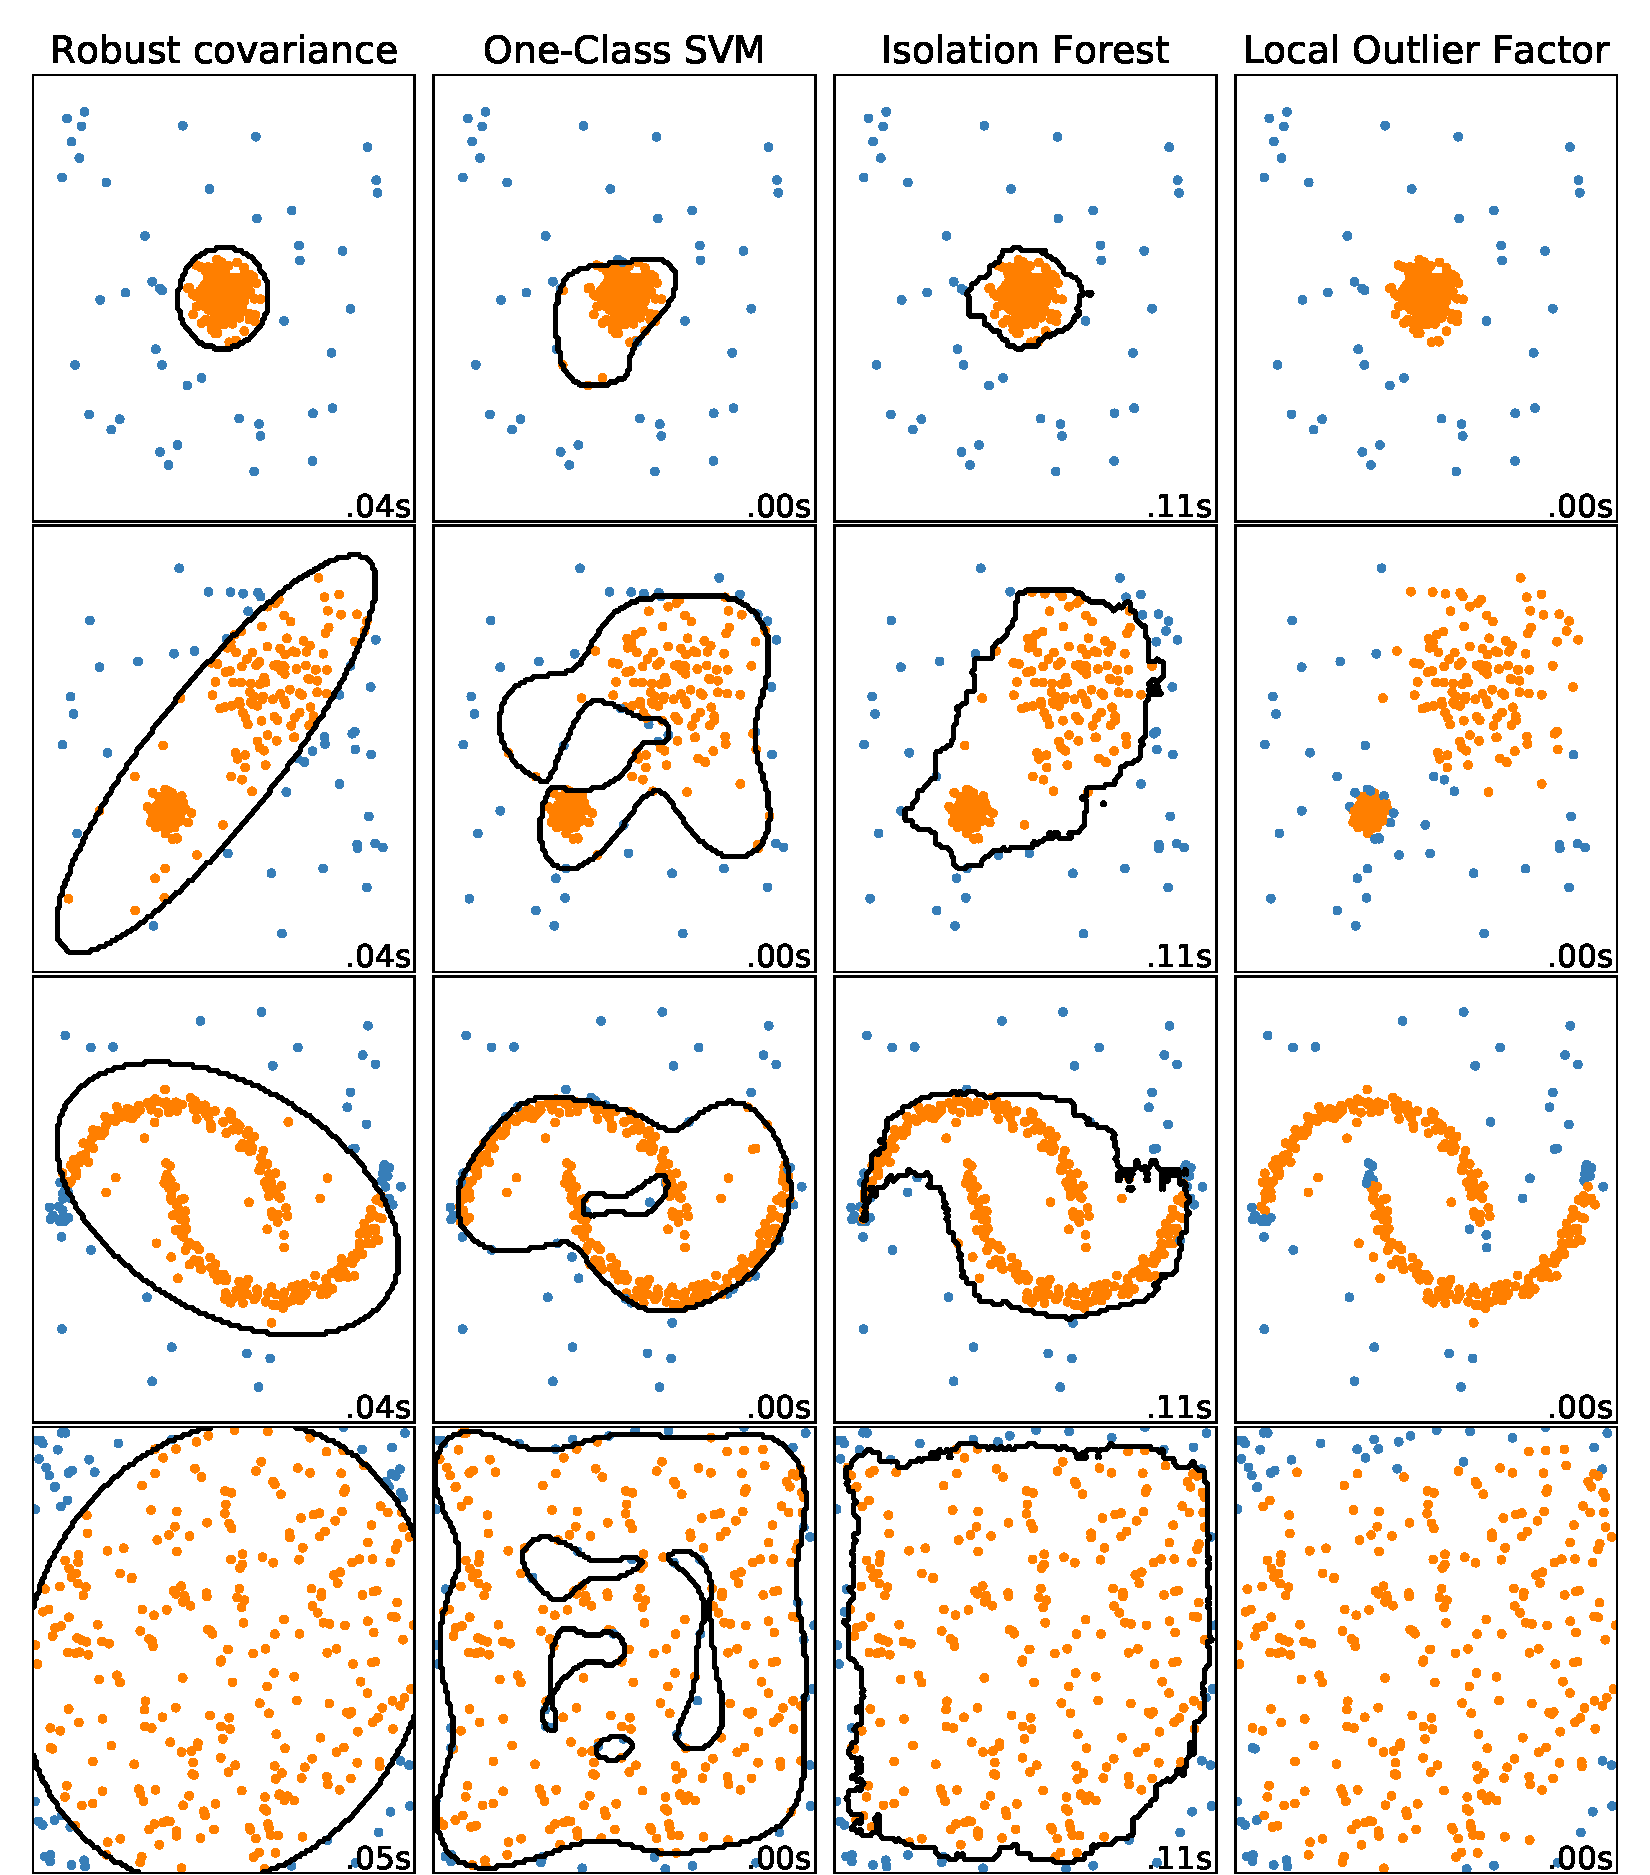
\includegraphics[width=6.8cm]{img/anomaly_comparison.pdf}
\end{center}

\end{frame}


\begin{frame}\frametitle{Scikit-learn API}

PR on \textbf{outlier detection API consistency} $\vcenter{\hbox{
\includegraphics[width=1.7cm]{img/merged_logo.pdf}}}$ last week

\begin{itemize}
  \item instantiate your estimator, e.g.~\mintinline{python}{clf = OneClassSVM()}
  \item \mintinline{python}{clf.fit(X)}
  \item raw score $s$ given by \mintinline{python}{clf.score_samples(X)}
  \item thresholded score \mintinline{python}{clf.decision_function(X)}
  \begin{equation*}
  \begin{cases}
    \text{\mintinline{python}{clf.decision_function(X)}} \geq 0 \quad \text{for inliers} \\
     \text{\mintinline{python}{clf.decision_function(X)}} < 0 \quad \text{for outliers}
  \end{cases}
  \end{equation*}
  \item \mintinline{python}{clf.predict(X)}
\end{itemize}
\end{frame}


\end{document}



